% Provenance (never printed): see sources/outline_sources.md and sources/book1/BRIEFS.md (g4/02).
\chapter{Programs and the Operating System}\label{ch:g4:programs-and-operating-system}

Lina wants to play on her tablet, but its screen shows only a bar that fills
slowly, and the word ``updating''. She cannot do anything but wait, so she
picks up a book. What is being changed inside the tablet? Who decided to change
it? And what is the tablet doing during all that time?

\begin{omfigure}
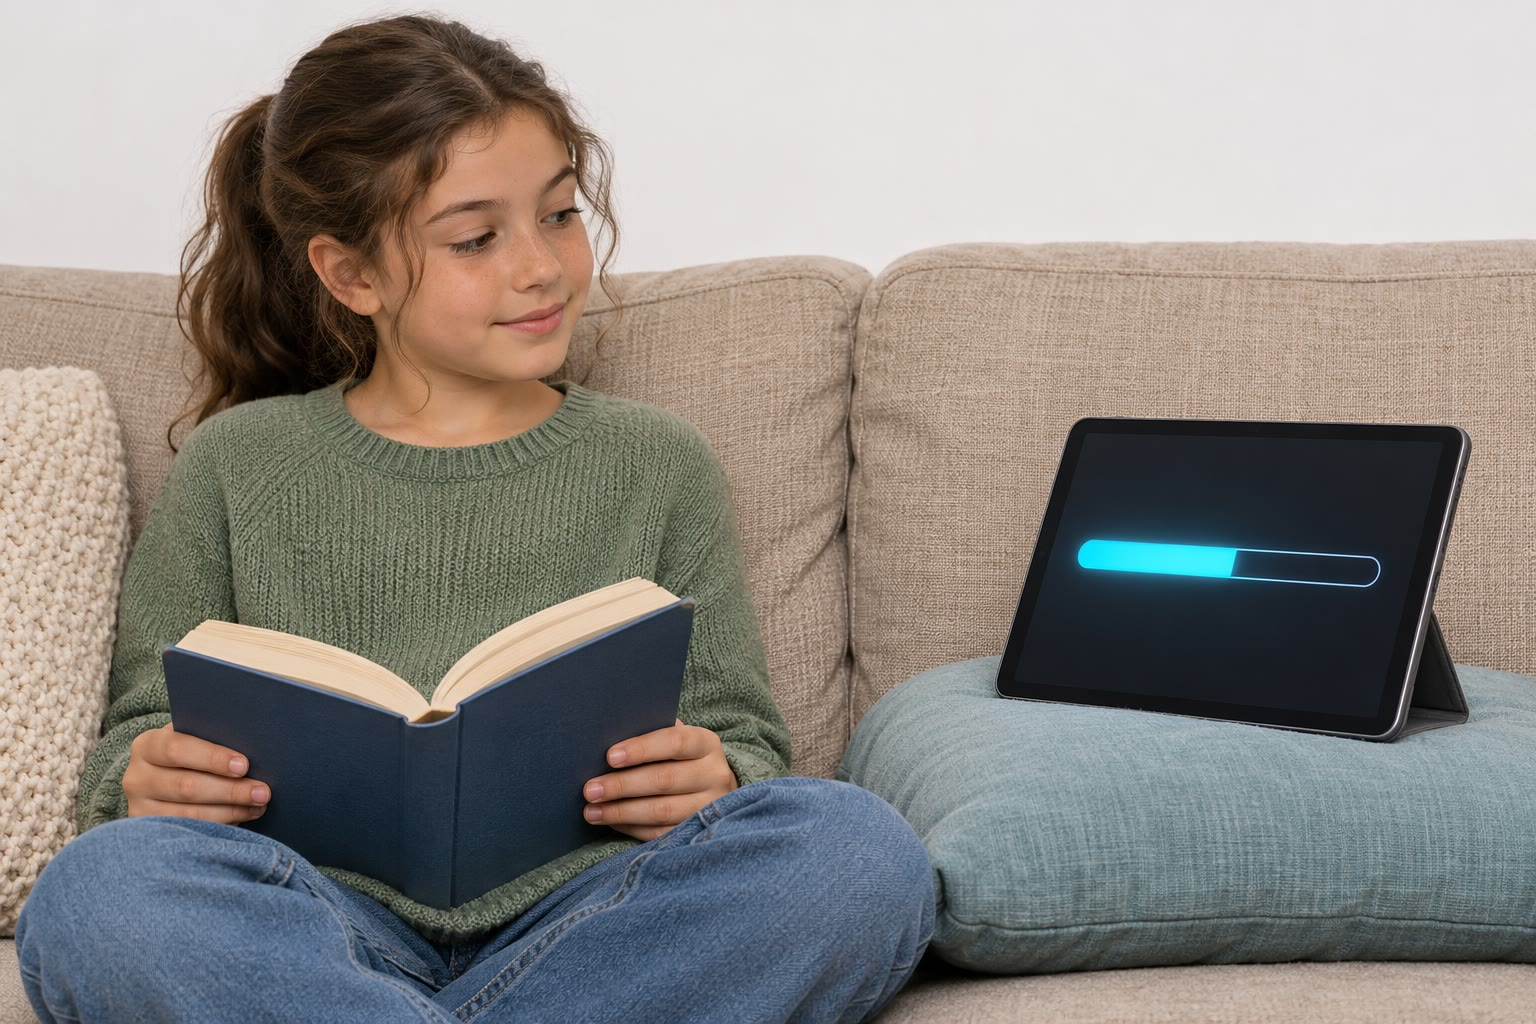
\includegraphics[width=0.52\linewidth]{images/book1/ai/g4-programs-and-operating-system-update.jpg}

{\small Waiting for an \omterm{def:g4:programs-and-operating-system:install}{update} to finish.}
\end{omfigure}

\begin{recall}
The \omterm{def:g3:inside-the-computer:processor}{processor} carries out \omterm{def:g1:instructions-in-order:instruction}{instructions}; the \omterm{def:g3:inside-the-computer:memory}{memory} holds the work in progress;
the \omterm{def:g3:inside-the-computer:storage}{storage} keeps \omterm{def:g3:files-and-folders:file}{files} (\cref{ch:g3:inside-the-computer,ch:g3:files-and-folders}).
Each piece of work is opened in a window (\cref{ch:g2:using-a-computer}).
\end{recall}

\section{A program is a list of instructions}

\begin{definition}[Program]\label{def:g4:programs-and-operating-system:program}
A \emph{program}\index{program} is a list of \omterm{def:g1:instructions-in-order:instruction}{instructions} for a \omterm{def:g1:what-is-a-computer:computer}{computer},
written by people and kept as a \omterm{def:g3:files-and-folders:file}{file}. The \omterm{def:g3:inside-the-computer:processor}{processor} carries out its
\omterm{def:g1:instructions-in-order:instruction}{instructions} one after another.
\end{definition}

A \omterm{def:g4:programs-and-operating-system:program}{program} is kept in the \omterm{def:g3:inside-the-computer:storage}{storage}, like any other \omterm{def:g3:files-and-folders:file}{file}. To run it, the \omterm{def:g1:what-is-a-computer:computer}{computer}
copies it into the \omterm{def:g3:inside-the-computer:memory}{memory}, because the \omterm{def:g3:inside-the-computer:processor}{processor} reads its \omterm{def:g1:instructions-in-order:instruction}{instructions} from
the \omterm{def:g3:inside-the-computer:memory}{memory}, where they can be reached quickly. A game, a \omterm{def:g2:using-a-computer:word-processor}{text editor} and a
drawing tool are all \omterm{def:g4:programs-and-operating-system:program}{programs}. A photo or a story is not a \omterm{def:g4:programs-and-operating-system:program}{program}: it is not
a list of \omterm{def:g1:instructions-in-order:instruction}{instructions}, it is information that a \omterm{def:g4:programs-and-operating-system:program}{program} works on.

\section{Applications}

\begin{definition}[Application]\label{def:g4:programs-and-operating-system:application}
An \emph{application}\index{application} is a \omterm{def:g4:programs-and-operating-system:program}{program} made for one task of
its user: drawing, writing, playing a game, listening to music, visiting web
pages.
\end{definition}

One \omterm{def:g4:programs-and-operating-system:application}{application} can be opened in several windows at once: two stories in two
windows of the same \omterm{def:g2:using-a-computer:word-processor}{word processor}, for example. Several \omterm{def:g4:programs-and-operating-system:application}{applications} can also
run at the same time: music plays while you write.

\section{The operating system}

When Lina saves a drawing, the drawing \omterm{def:g4:programs-and-operating-system:application}{application} does not drive the \omterm{def:g3:inside-the-computer:storage}{storage}
itself. It asks another \omterm{def:g4:programs-and-operating-system:program}{program} to do it.

\begin{definition}[Operating system]\label{def:g4:programs-and-operating-system:os}
The \emph{operating system}\index{operating system} is the \omterm{def:g4:programs-and-operating-system:program}{program} that
starts first when a \omterm{def:g1:what-is-a-computer:computer}{computer} is switched on and runs all the others. It looks
after the \omterm{def:g3:files-and-folders:file}{files}, shares the \omterm{def:g3:inside-the-computer:memory}{memory} and the \omterm{def:g3:inside-the-computer:processor}{processor} between the \omterm{def:g4:programs-and-operating-system:program}{programs},
drives the \omterm{def:g3:inside-the-computer:device}{devices}, and keeps the users apart.
\end{definition}

\begin{omfigure}
\begin{tikzpicture}[x=1cm, y=1cm, font=\footnotesize,
    layer/.style={draw=black!60, rounded corners=2pt, minimum width=7cm, minimum height=0.9cm, align=center, font=\small}]
  \node[layer, fill=ocYellow!35] (u) at (0,4.5) {the user};
  \node[layer, fill=ocMint!30] (a) at (0,3.0) {applications\\{\footnotesize drawing, writing, games, browser}};
  \node[layer, fill=ocBlue!25] (o) at (0,1.5) {operating system};
  \node[layer, fill=black!10] (h) at (0,0) {hardware\\{\footnotesize processor, memory, storage, devices}};
  \foreach \x/\y/\t in {u/a/{``save my drawing''}, a/o/{``write this file''}, o/h/{``store these bytes''}} {
    \draw[-{Stealth[length=2mm]}, ocRed!80!black, thick] ([xshift=-1.2cm]\x.south) -- node[left, font=\footnotesize, text=ocRed!80!black] {\t} ([xshift=-1.2cm]\y.north);
  }
  \foreach \x/\y/\t in {h/o/{done}, o/a/{done}, a/u/{``saved''}} {
    \draw[-{Stealth[length=2mm]}, ocBlue!80!black, thick] ([xshift=1.2cm]\x.north) -- node[right, font=\footnotesize, text=ocBlue!80!black] {\t} ([xshift=1.2cm]\y.south);
  }
\end{tikzpicture}

{\small The layers of a \omterm{def:g1:what-is-a-computer:computer}{computer}. A request goes down, one layer at a time,
and the answer comes back up. The user talks to the \omterm{def:g4:programs-and-operating-system:application}{applications}, the
\omterm{def:g4:programs-and-operating-system:application}{applications} ask the \omterm{def:g4:programs-and-operating-system:os}{operating system}, and only the \omterm{def:g4:programs-and-operating-system:os}{operating system} drives
the hardware.}
\label{fig:g4:programs-and-operating-system:layers}
\end{omfigure}

\begin{omfigure}
\begin{tikzpicture}[x=1cm, y=1cm, font=\footnotesize,
    job/.style={draw=black!60, fill=ocMint!25, rounded corners=2pt, minimum width=2.7cm, minimum height=0.8cm, align=center}]
  \node[draw=black!70, fill=ocBlue!25, rounded corners=3pt, minimum width=3.2cm, minimum height=1cm, font=\small] (os) at (0,0) {operating system};
  \node[job] (f) at (-4.6,1.3) {files\\{\scriptsize folders, saving, opening}};
  \node[job] (m) at (4.6,1.3) {memory and processor\\{\scriptsize shared between programs}};
  \node[job] (d) at (-4.6,-1.3) {devices\\{\scriptsize keyboard, screen, printer}};
  \node[job] (us) at (4.6,-1.3) {users\\{\scriptsize accounts and passwords}};
  \foreach \n in {f,m,d,us} \draw[-{Stealth[length=2mm]}, thick, black!60] (os) -- (\n);
\end{tikzpicture}

{\small The four things an \omterm{def:g4:programs-and-operating-system:os}{operating system} looks after.}
\label{fig:g4:programs-and-operating-system:jobs}
\end{omfigure}

A \omterm{def:g1:what-is-a-computer:computer}{computer} used by several people keeps their work apart.

\begin{definition}[User account]\label{def:g4:programs-and-operating-system:account}
A \emph{user account}\index{user account} is the place an \omterm{def:g4:programs-and-operating-system:os}{operating system}
keeps for one person: a name, a password, the person's own \omterm{def:g3:files-and-folders:folder}{folders} and
settings. The \omterm{def:g4:programs-and-operating-system:os}{operating system} lets each person open only their own account.
\end{definition}

\begin{dated}{2026}
% ledger: g4:os-windows, g4:os-macos, g4:os-linux, g4:os-chromeos, g4:os-android, g4:os-ios, g4:os-ipados
The main families of \omterm{def:g4:programs-and-operating-system:os}{operating systems} in 2026: Windows, macOS, Linux and
ChromeOS on desktop \omterm{def:g1:what-is-a-computer:computer}{computers} and laptops; Android, iOS and iPadOS on phones
and tablets. Each family keeps changing: the makers bring out new versions
and send \omterm{def:g4:programs-and-operating-system:install}{updates}.
\end{dated}

\section{Starting up}

\begin{definition}[Start-up]\label{def:g4:programs-and-operating-system:startup}
The \emph{start-up}\index{start-up} of a \omterm{def:g1:what-is-a-computer:computer}{computer} is what happens between
pressing the power button and the moment the \omterm{def:g1:what-is-a-computer:computer}{computer} is ready to use: a small
\omterm{def:g4:programs-and-operating-system:program}{program} kept on the \omterm{def:g3:inside-the-computer:motherboard}{motherboard} checks the parts and starts the \omterm{def:g4:programs-and-operating-system:os}{operating
system} from the \omterm{def:g3:inside-the-computer:storage}{storage}.
\end{definition}

\begin{omfigure}
\begin{tikzpicture}[x=1cm, y=1cm, font=\footnotesize,
    st/.style={draw=black!60, fill=ocYellow!30, rounded corners=2pt, text width=3.6cm, minimum height=1.2cm, align=center}]
  \foreach \t [count=\i] in {press the power button,
      a small program on the motherboard checks the parts,
      it finds the operating system in the storage,
      the operating system is copied into memory,
      the operating system starts its services,
      the login screen or the desktop appears} {
    \node[st] (s\i) at ({4.4*mod(\i-1,3)}, {-1.9*int((\i-1)/3)}) {\i.~\t};
  }
  \foreach \a/\b in {1/2, 2/3, 4/5, 5/6} \draw[-{Stealth[length=2mm]}, thick, black!60] (s\a) -- (s\b);
  \draw[-{Stealth[length=2mm]}, thick, black!60] (s3.south) -- ++(0,-0.18) -| (s4.north);
\end{tikzpicture}

{\small The \omterm{def:g4:programs-and-operating-system:startup}{start-up} of a \omterm{def:g1:what-is-a-computer:computer}{computer}, step by step. It takes a few seconds.}
\label{fig:g4:programs-and-operating-system:startup}
\end{omfigure}

\section{Installing and updating}

\begin{definition}[Installing and updating]\label{def:g4:programs-and-operating-system:install}
To \emph{install}\index{installation (of a program)} a \omterm{def:g4:programs-and-operating-system:program}{program} is to copy its
\omterm{def:g3:files-and-folders:file}{files} into the \omterm{def:g3:inside-the-computer:storage}{storage} of a \omterm{def:g1:what-is-a-computer:computer}{computer} and to tell the \omterm{def:g4:programs-and-operating-system:os}{operating system} about it,
so that it can be started. To \emph{update}\index{update (of a program)} a
\omterm{def:g4:programs-and-operating-system:program}{program} is to replace some of its \omterm{def:g3:files-and-folders:file}{files} by newer ones.
\end{definition}

\omterm{def:g4:programs-and-operating-system:program}{Programs} are written by people, and people make mistakes. Some mistakes make
a \omterm{def:g4:programs-and-operating-system:program}{program} stop or give wrong results; others leave a hole that a stranger
could use to get into the \omterm{def:g1:what-is-a-computer:computer}{computer}. When the makers find a mistake, they send
an \omterm{def:g4:programs-and-operating-system:install}{update} that fixes it. This is what Lina's tablet was doing: its \omterm{def:g4:programs-and-operating-system:os}{operating
system} was replacing some of its own \omterm{def:g3:files-and-folders:file}{files} by better ones, and the tablet
could not be used while those \omterm{def:g3:files-and-folders:file}{files} were being changed.

\begin{safety}
Accept the \omterm{def:g4:programs-and-operating-system:install}{updates} of your \omterm{def:g4:programs-and-operating-system:os}{operating system} and your \omterm{def:g4:programs-and-operating-system:application}{applications}: many of
them close holes that strangers could use. \omterm{def:g4:programs-and-operating-system:install}{Install} \omterm{def:g4:programs-and-operating-system:program}{programs} only from the
places your \omterm{def:g3:inside-the-computer:device}{device} or your school trusts, never from a message or a website
that offers one out of nowhere.
\end{safety}

\section{Exercises}

\begin{exercise}[$\star$]\label{exo:g4:programs-and-operating-system:1}
Is it a \omterm{def:g4:programs-and-operating-system:program}{program}? A recipe card, a game, a photo, a \omterm{def:g2:using-a-computer:word-processor}{text editor}.
\end{exercise}

\begin{exercise}[$\star$]\label{exo:g4:programs-and-operating-system:2}
Give three things the \omterm{def:g4:programs-and-operating-system:os}{operating system} looks after.
\end{exercise}

\begin{exercise}[$\star$]\label{exo:g4:programs-and-operating-system:3}
Where is a \omterm{def:g4:programs-and-operating-system:program}{program} kept when the \omterm{def:g1:what-is-a-computer:computer}{computer} is switched off?
\end{exercise}

\begin{exercise}[$\star$]\label{exo:g4:programs-and-operating-system:4}
Put the steps of a \omterm{def:g4:programs-and-operating-system:startup}{start-up} in order: (a)~the \omterm{def:g4:programs-and-operating-system:os}{operating system} is copied into
\omterm{def:g3:inside-the-computer:memory}{memory}; (b)~the power button is pressed; (c)~the login screen appears; (d)~a
small \omterm{def:g4:programs-and-operating-system:program}{program} on the \omterm{def:g3:inside-the-computer:motherboard}{motherboard} checks the parts; (e)~the \omterm{def:g4:programs-and-operating-system:os}{operating system}
is found in the \omterm{def:g3:inside-the-computer:storage}{storage}.
\end{exercise}

\begin{exercise}[$\star$]\label{exo:g4:programs-and-operating-system:5}
Give two reasons to accept \omterm{def:g4:programs-and-operating-system:install}{updates}.
\end{exercise}

\begin{exercise}[$\star$]\label{exo:g4:programs-and-operating-system:6}
Follow the drawing of the layers for ``print this page'': what does each layer
ask the one below?
\end{exercise}

\begin{exercise}[$\star$]\label{exo:g4:programs-and-operating-system:7}
\omterm{def:g4:programs-and-operating-system:application}{Application} or \omterm{def:g4:programs-and-operating-system:os}{operating system}? (a)~Drawing a cat. (b)~Sharing the \omterm{def:g3:inside-the-computer:memory}{memory}
between two \omterm{def:g4:programs-and-operating-system:program}{programs}. (c)~Checking the spelling of a story. (d)~Showing the
login screen. (e)~Sending \omterm{def:g4:memory-and-storage:byte}{bytes} to the printer.
\end{exercise}

\begin{exercise}[$\star\star$]\label{exo:g4:programs-and-operating-system:8}
Lina and her brother use the same \omterm{def:g1:what-is-a-computer:computer}{computer}, each with a \omterm{def:g4:programs-and-operating-system:account}{user account}. What does
the \omterm{def:g4:programs-and-operating-system:os}{operating system} keep apart? Why is that useful?
\end{exercise}

\begin{exercise}[$\star\star$]\label{exo:g4:programs-and-operating-system:9}
Why is a \omterm{def:g4:programs-and-operating-system:program}{program} copied from the \omterm{def:g3:inside-the-computer:storage}{storage} into the \omterm{def:g3:inside-the-computer:memory}{memory} before it runs?
\end{exercise}

\begin{exercise}[$\star\star$]\label{exo:g4:programs-and-operating-system:10}
While Tom visits a website, a window appears: ``Your \omterm{def:g1:what-is-a-computer:computer}{computer} is slow!
Download this \omterm{def:g4:programs-and-operating-system:install}{update} now.'' What should he do, and why?
\end{exercise}
